\documentclass{standalone}

\usepackage{tikz,tikz-3dplot, tkz-euclide}
\usetikzlibrary{arrows.meta}
\usetikzlibrary{calc}
\tikzset{>={Latex[round]}}
\usetikzlibrary{math}

\usepackage{relsize} % mathsmaller
\usepackage{amsmath}
\usepackage{mathtools} %boldsymbol

\usepackage{pgfplots}
\pgfplotsset{compat=1.12}
\usetikzlibrary{backgrounds}

\begin{document}
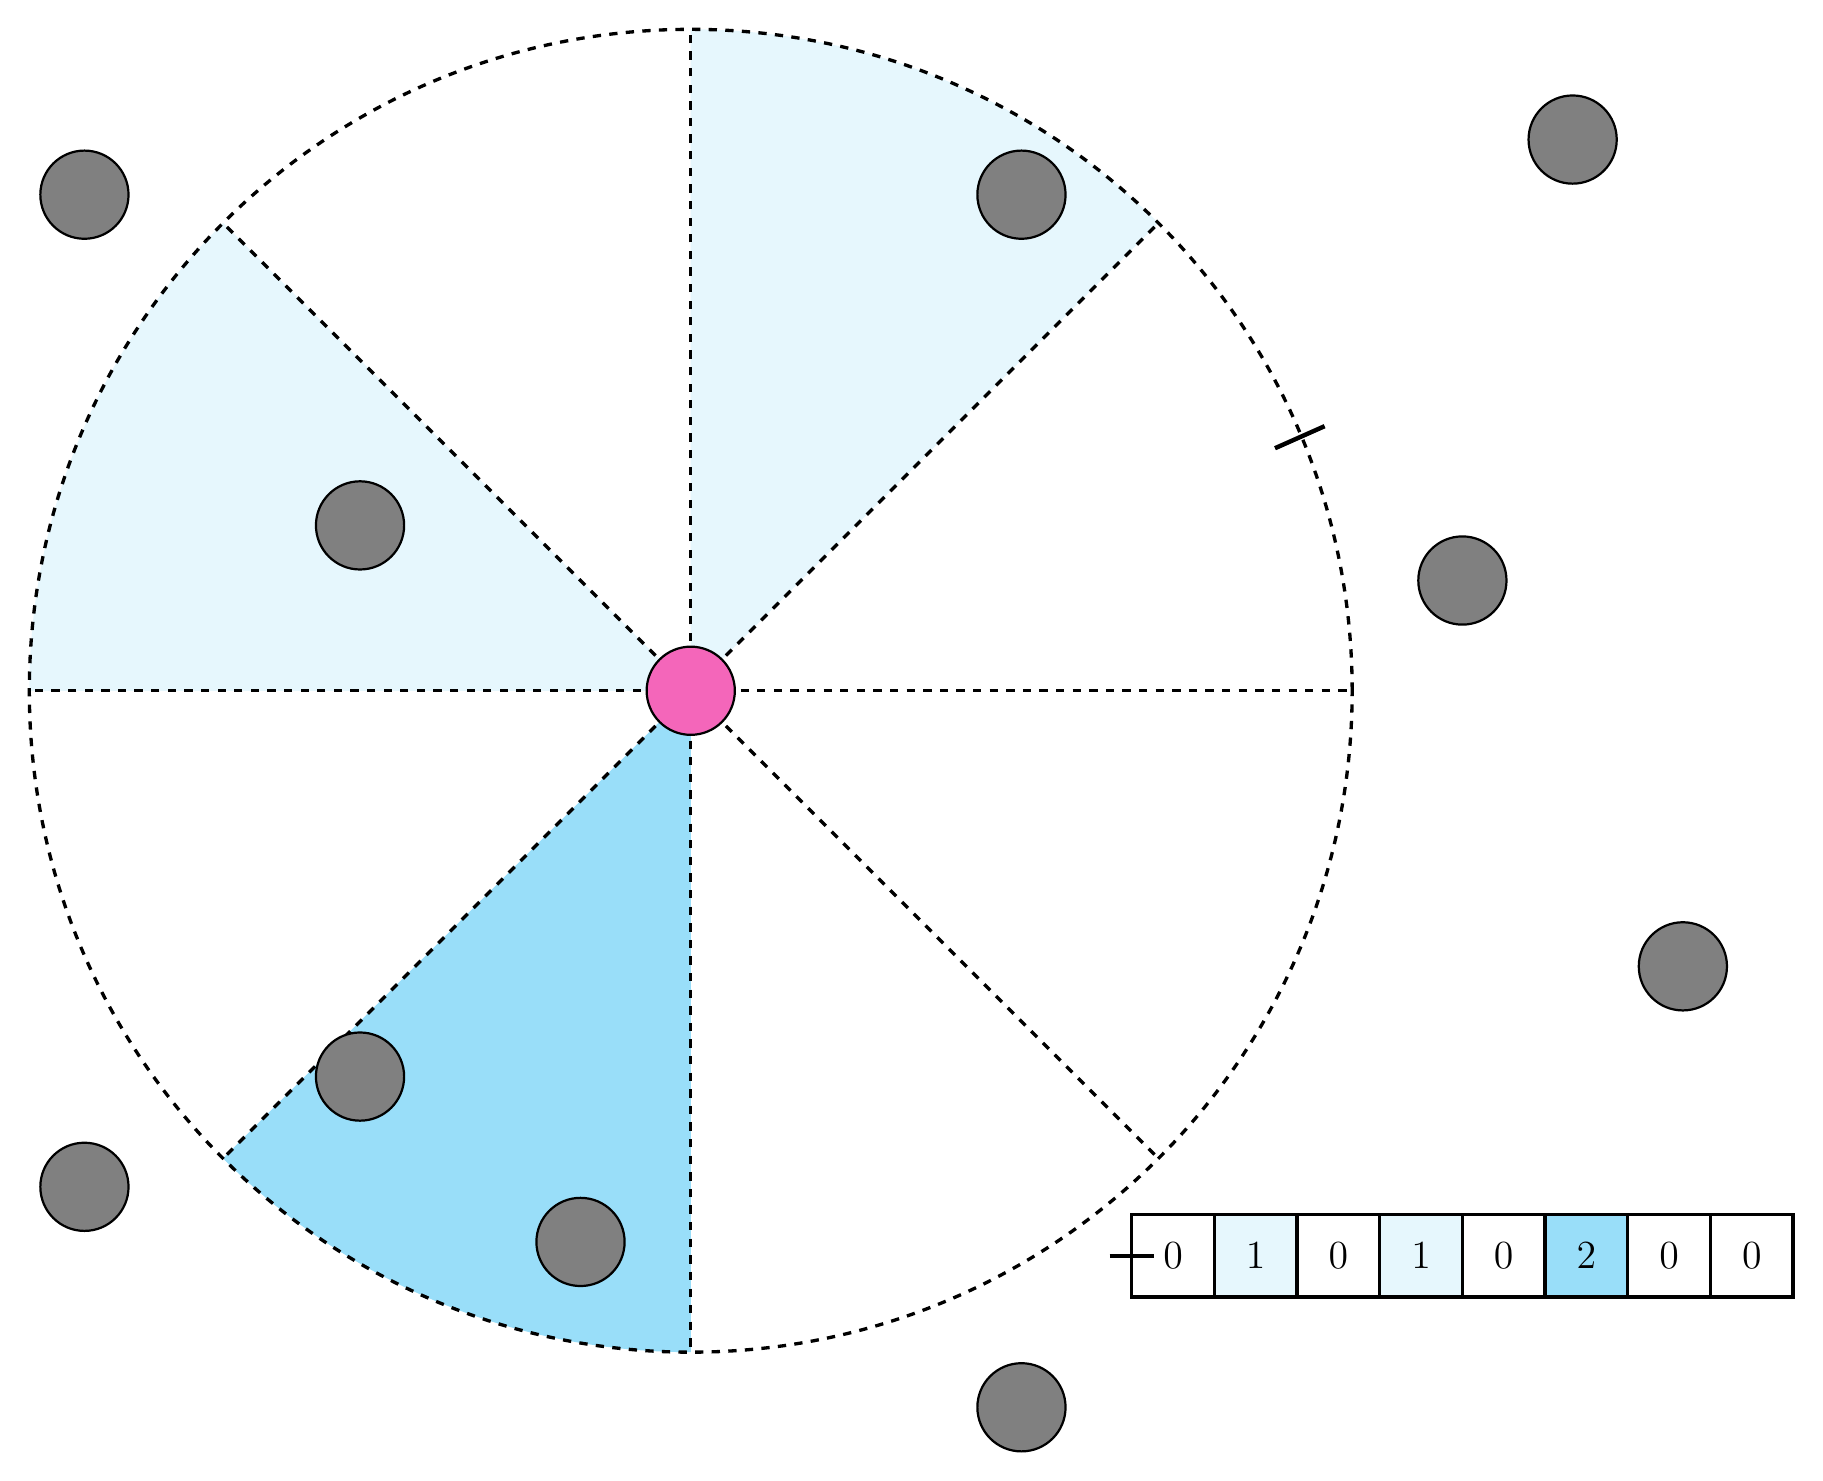
\begin{tikzpicture}[scale=7]

\fill[cyan!10] (0,0) --  (45:1.2) arc(45:90:1.2);
\fill[cyan!10] (0,0) --  (135:1.2) arc(135:180:1.2);
\fill[cyan!40] (0,0) --  (225:1.2) arc(225:270:1.2);

\draw[very thick, dashed] (0,0) -- (1.2, 0);
\draw[very thick, dashed] (0,0) -- (0.85, 0.85);
\draw[very thick, dashed] (0,0) -- (0, 1.2);
\draw[very thick, dashed] (0,0) -- (-0.85, 0.85);
\draw[very thick, dashed] (0,0) -- (-1.2, 0);
\draw[very thick, dashed] (0,0) -- (-0.85, -0.85);
\draw[very thick, dashed] (0,0) -- (0, -1.2);
\draw[very thick, dashed] (0,0) -- (0.85, -0.85);

\draw[very thick, dashed] (0,0) circle (1.2);

\draw[thick, fill=magenta!60] (0,0) circle (0.08);

\draw[thick, fill=gray] (1.6, 1) circle (0.08);
\draw[thick, fill=gray] (1.4, 0.2) circle (0.08);
\draw[thick, fill=gray] (-1.1, 0.9) circle (0.08);
\draw[thick, fill=gray] (-1.1, -0.9) circle (0.08);
\draw[thick, fill=gray] (0.6, -1.3) circle (0.08);
\draw[thick, fill=gray] (1.8, -0.5) circle (0.08);

\draw[thick, fill=gray] (0.6, 0.9) circle (0.08);
\draw[thick, fill=gray] (-0.6, 0.3) circle (0.08);
\draw[thick, fill=gray] (-0.2, -1.0) circle (0.08);
\draw[thick, fill=gray] (-0.6, -0.7) circle (0.08);

\draw[very thick] (0.8,-1.1) rectangle node {\Large{0}} ++(0.15, 0.15);
\draw[very thick, fill=cyan!10] (0.95,-1.1) rectangle node {\Large{1}} ++(0.15, 0.15);
\draw[very thick] (1.1,-1.1) rectangle node {\Large{0}} ++(0.15, 0.15);
\draw[very thick, fill=cyan!10] (1.25,-1.1) rectangle node {\Large{1}} ++(0.15, 0.15);
\draw[very thick] (1.4,-1.1) rectangle node {\Large{0}} ++(0.15, 0.15);
\draw[very thick, fill=cyan!40] (1.55,-1.1) rectangle node {\Large{2}} ++(0.15, 0.15);
\draw[very thick] (1.7,-1.1) rectangle node {\Large{0}} ++(0.15, 0.15);
\draw[very thick] (1.85,-1.1) rectangle node {\Large{0}} ++(0.15, 0.15);

\draw[ultra thick, black] (1.06, 0.44) -- (1.15, 0.48);

\draw[ultra thick, black] (0.76, -1.025) -- (0.84, -1.025);

\end{tikzpicture}
\end{document}